\section{The Proposed Method -GAN network object detection method}
\label{segmethod}

In this section, we describe the process for object detection in using GAN network object detection method. The process consist of the following steps: blood smears image acquisition, image generation with GANs networks (Figure \ref{fig:maincomp} -\ding{202} ); train a convolutional neural network (Figure \ref{fig:maincomp} -\ding{203});  apply adaptive  threshold filter (Figure \ref{fig:maincomp} -\ding{204}) and classify objects with the trained convolutional network (Figure \ref{fig:maincomp} -\ding{205}). 

Several experiments where conducted in order to analyse the benefits of use GAN networks in the proposed method. The images for the experiments where acquired from the repository presented by Quinn et al. \cite{Quinn2016DeepDiagnostics}.  The code are developed in python language using the Keras framework.

The experiments used a Deep convolutional generative adversarial network according to the architecture shown in figure


\lstset{basicstyle=\footnotesize\ttfamily,breaklines=true}
\begin{lstlisting}[language=Python,numbers=left,frame=tb,caption=Generator Keras Code]
model = Sequential()

model.add(Dense(512 * 7* 7, activation="relu",     
input_dim=self.latent_dim))

model.add(Reshape((7,7, 512)))
model.add(UpSampling2D())
model.add(Conv2D(256, kernel_size=3, padding="same"))
model.add(BatchNormalization(momentum=0.8))
model.add(Activation("relu"))
model.add(UpSampling2D())
model.add(Conv2D(128, kernel_size=3, padding="same"))
model.add(BatchNormalization(momentum=0.8))
model.add(Activation("relu"))
model.add(UpSampling2D())
model.add(Conv2D(64, kernel_size=3, padding="same"))
model.add(BatchNormalization(momentum=0.8))
model.add(Activation("relu"))
model.add(UpSampling2D())
model.add(Conv2D(32, kernel_size=3, padding="same"))
model.add(BatchNormalization(momentum=0.8))
model.add(Activation("relu"))
model.add(Conv2D(self.channels, 
            kernel_size=3, padding="same"))
model.add(Activation("tanh"))

model.summary()

noise = Input(shape=(self.latent_dim,))
img = model(noise)

\end{lstlisting}


\begin{figure*}[h]
\caption{Main components of the proposed method .}
\label{fig:maincomp}
  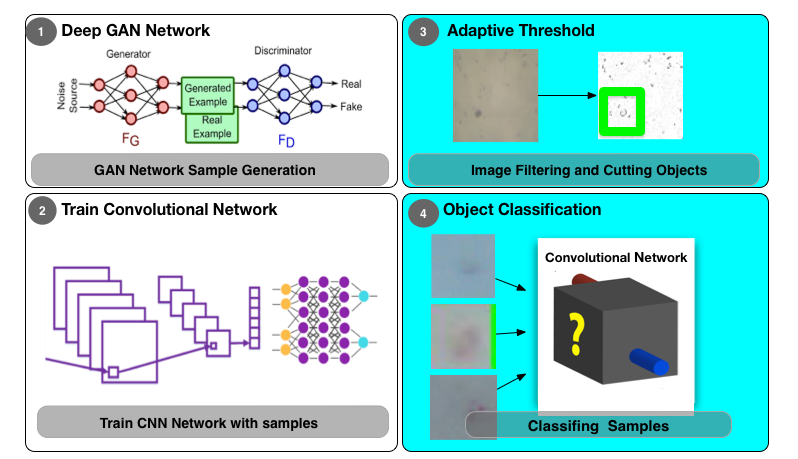
\includegraphics[width=\textwidth]{images/MainComponents.png}
  
\end{figure*}



\begin{figure}[h]
\caption{Main components of the proposed method .}
\label{fig:gen50}
\begin{center}
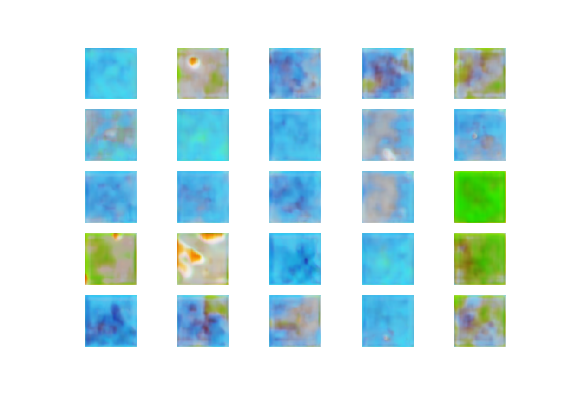
\includegraphics[scale=0.45]{./images/generation/alta_mnist_50.png} \end{center}\caption{Generated images after 50 epochs}
\end{figure}

\begin{figure}[h]
\caption{Generated images after 250 epochs}
\label{fig:gen250}
\begin{center}
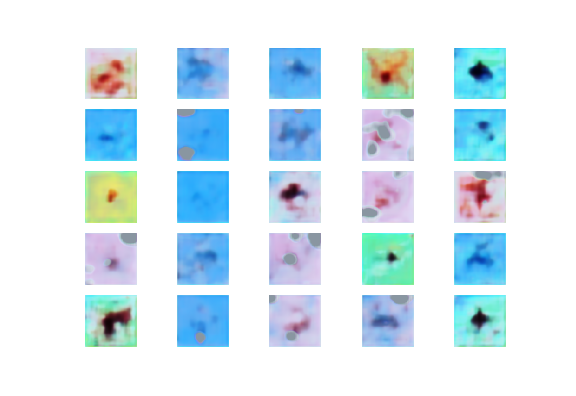
\includegraphics[scale=0.45]{./images/generation/alta_mnist_250.png} \end{center}

\end{figure}


\begin{figure}[h]
\label{fig:gen30410}
\begin{center}
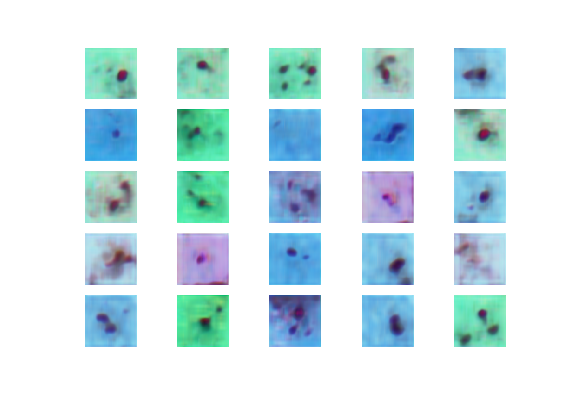
\includegraphics[scale=0.45]{./images/generation/alta_mnist_30410.png} \end{center}
\caption{Generated images after 30410 epochs}
\end{figure}



\begin{figure*}[htp]
  \centering
  \subfigure[random caption 1]{
  %\caption{Generated images after 30410 epochs}
  %\label{fig:threshold}
  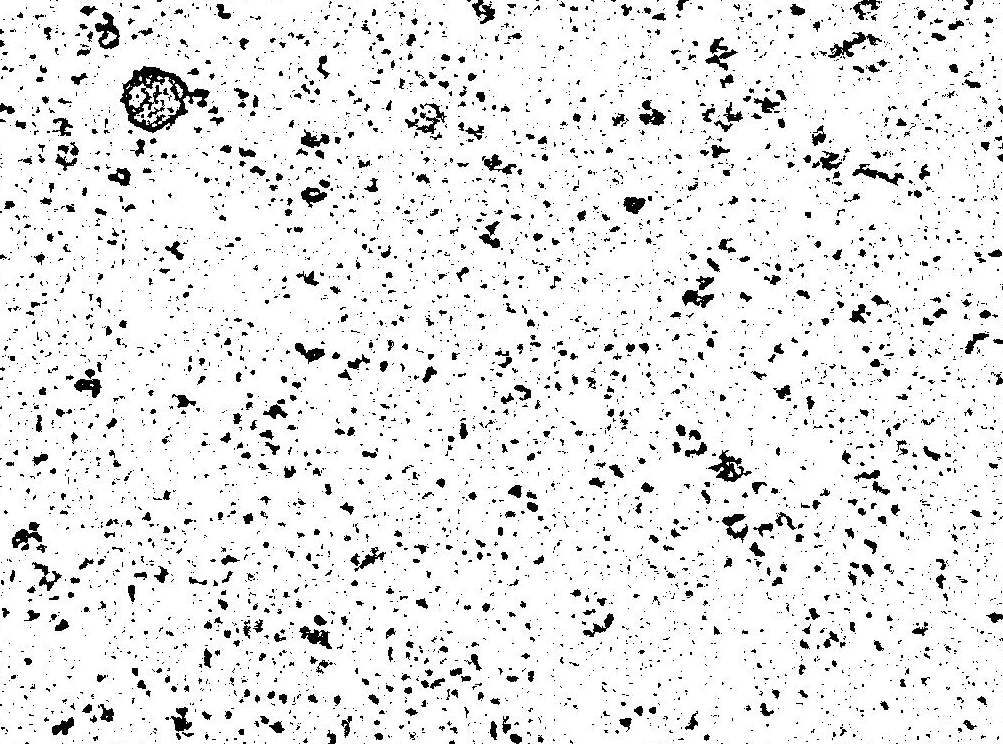
\includegraphics[scale=0.21]{./images/threshold.png}
  }
  \subfigure[random caption 2]{
  %\caption{Generated images after 30410 epochs}
  %\label{fig:objectdetect}
  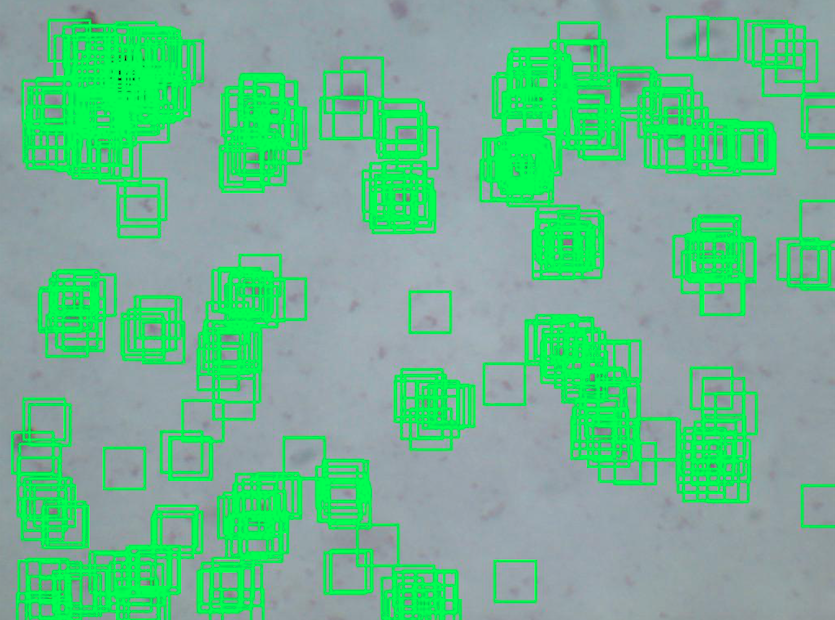
\includegraphics[scale=0.25]{./images/object_detected.png}
  }
\end{figure*}


% Please add the following required packages to your document preamble:
% \usepackage[table,xcdraw]{xcolor}
% If you use beamer only pass "xcolor=table" option, i.e. \documentclass[xcolor=table]{beamer}
\begin{table}[h]
\caption{Results of training the CNN network with images generates by DGAN network}
\label{tab:results}
\begin{tabular}{|l|l|l|l|}
\hline
\rowcolor[HTML]{C0C0C0} 
\textbf{\begin{tabular}[c]{@{}l@{}}Number of \\ Samples \\ Created\\ by GAN \\ Network\end{tabular}} & \textbf{\begin{tabular}[c]{@{}l@{}}Number of\\ Real \\ Images\\ for Test\end{tabular}} & \textbf{\begin{tabular}[c]{@{}l@{}}Number \\ of correctly \\ classified \\ samples\end{tabular}} & \textbf{\begin{tabular}[c]{@{}l@{}}Number of \\ incorrectly \\ classified \\ samples\end{tabular}} \\ \hline
600                                                                                            & 600                                                                                 & 420 (70 \%)                                                                                      & 180                                                                                                \\ \hline
800                                                                                            & 600                                                                                 & 406 (68 \%)                                                                                      & 194                                                                                                \\ \hline
1000                                                                                           & 600                                                                                 & 453 (76 \%)                                                                                      & 147                                                                                                \\ \hline
1200                                                                                           & 600                                                                                 & 424 (71 \%)                                                                                      & 176                                                                                                \\ \hline
1400                                                                                           & 600                                                                                 & \begin{tabular}[c]{@{}l@{}}429 \\ ($\sim$71 \%)\end{tabular}                                     & 171                                                                                                \\ \hline
1600                                                                                           & 600                                                                                 & 430 (72 \%)                                                                                      & 170                                                                                                \\ \hline
1800                                                                                           & 600                                                                                 & 480 (80  \%)                                                                                     & 120                                                                                                \\ \hline
2200                                                                                           & 600                                                                                 & 600 (100 \%)                                                                                     & 0                                                                                                  \\ \hline
\end{tabular}
\end{table}

